\documentclass[../../main.tex]{subfiles}
\begin{document}

{\bf [解答]}

三次元$xyz$空間において$A(a,0,0)$， $B(0,b,0)$， $C(0,0,c)$ とおく．
四面体$ABCD$は全ての面が合同であることと対称性から，$D(a,b,c)$ の時のみ考えれば良い．

\begin{figure}[htb]
  \centering
  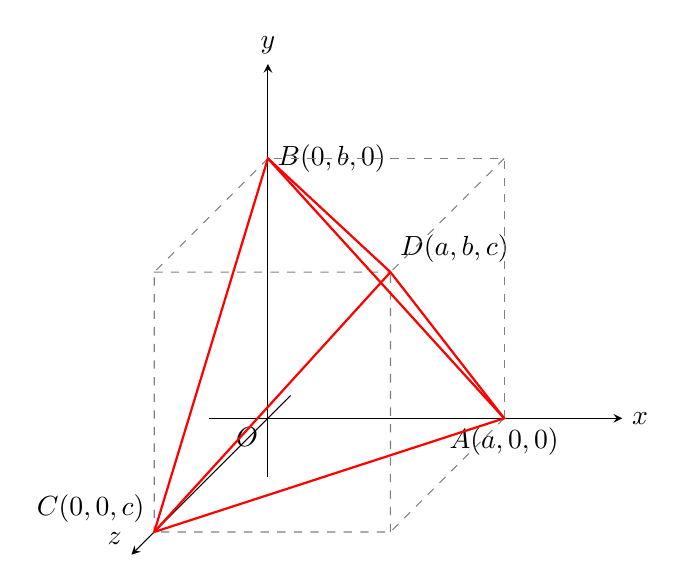
\begin{tikzpicture}[scale=1.5, >=stealth]
    % Axes
    \draw[->] (-0.5,0,0) -- (3,0,0) node[right] {$x$};
    \draw[->] (0,-0.5,0) -- (0,3,0) node[above] {$y$};
    \draw[->] (0,0,-0.5) -- (0,0,3) node[above left] {$z$};

    \node[below left] at (0,0,0) {$O$};

    \coordinate (A) at (2,0,0);
    \coordinate (B) at (0,2.2,0);
    \coordinate (C) at (0,0,2.5);
    \coordinate (D) at (2,2.2,2.5);

    \node[below] at (A) {$A(a,0,0)$};
    \node[right] at (B) {$B(0,b,0)$};
    \node[above left] at (C) {$C(0,0,c)$};
    \node[above right] at (D) {$D(a,b,c)$};

    \draw[dashed, gray] (2,0,0) -- (2,2.2,0) -- (0,2.2,0);
    \draw[dashed, gray] (2,0,0) -- (2,0,2.5) -- (0,0,2.5);
    \draw[dashed, gray] (0,2.2,0) -- (0,2.2,2.5) -- (0,0,2.5);
    \draw[dashed, gray] (2,2.2,0) -- (D) (2,0,2.5) -- (D) (0,2.2,2.5) -- (D);

    \draw[thick, red] (A) -- (B) -- (C) -- cycle;
    \draw[thick, red] (A) -- (D);
    \draw[thick, red] (B) -- (D);
    \draw[thick, red] (C) -- (D);
  \end{tikzpicture}
  \caption{辺の長さが $a,b,c$ の直方体に内接する四面体 $ABCD$}
\end{figure}

上図のように3辺の長さが $a,b,c$ である直方体を考えると，
四面体$ABCD$の体積$V(l)$はこの直方体の体積から$4$つの体積$\dfrac{abc}{6}$の三角錐を取り除いたもので
\begin{align}
  V(l) = abc - 4 \cdot \dfrac{1}{6} abc = \dfrac{1}{3} abc \label{eq:1}
\end{align}
である．

そこで以下，$abc$を$l$で表すことを考える．
題意より$|AB| = 2l-1$， $|BC| = 2l$， $|CA| = 2l+1$ だから
ピタゴラスの定理より，
\begin{align}
  \begin{cases}
    (2l-1)^2 = a^2+b^2 \\
    (2l)^2 = b^2+c^2   \\
    (2l+1)^2 = a^2+c^2
  \end{cases} \label{eq:2}
\end{align}
である．各辺足し合わせて
\begin{align}
  12l^2+2 = 2(a^2+b^2+c^2) \implies 6l^2+1 = a^2+b^2+c^2
\end{align}
だから\cref{eq:2}から
\begin{align}
  a^2 = 2l^2+1, \quad b^2 = 2l^2-4l, \quad c^2 = 2l^2+4l \label{eq:3}
\end{align}
となる．
$a,b,c > 0$ に注意して\cref{eq:1}に代入すると
\begin{align}
  \dfrac{V(l)}{\sqrt{l-2}}
  &= \dfrac{1}{\sqrt{l-2}} \cdot \dfrac{1}{3} \sqrt{2l^2+1} \sqrt{2l(l-2)} \sqrt{2l(l+2)} \\
  &= \dfrac{2}{3} \sqrt{2l^2+1} \cdot \sqrt{l} \cdot \sqrt{l(l+2)} \\
  &\xrightarrow{l \to 2} \dfrac{8}{3}
\end{align}
が求める極限値である．

{\bf [解説]}

この解答では，直方体の対角線を結んで四面体 $ABCD$ をつくると全ての面が合同になるという事実を用いて解答を作った．
これはたびたび出てくるので覚えておくと良いだろう．

\begin{figure}[htb]
  \centering
  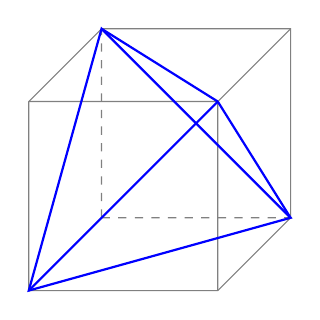
\begin{tikzpicture}[scale=1.2, >=stealth]
    % Cuboid vertices
    \coordinate (O) at (0,0,0);
    \coordinate (A) at (2,0,0);
    \coordinate (B) at (0,2,0);
    \coordinate (C) at (0,0,2);
    \coordinate (AB) at (2,2,0);
    \coordinate (BC) at (0,2,2);
    \coordinate (CA) at (2,0,2);
    \coordinate (D) at (2,2,2);

    % Draw cuboid edges
    \draw[gray, dashed] (O) -- (A) (O) -- (B) (O) -- (C);
    \draw[gray] (A) -- (AB) -- (B) (B) -- (BC) -- (C) (C) -- (CA) -- (A);
    \draw[gray] (AB) -- (D) (BC) -- (D) (CA) -- (D);

    % Tetrahedron edges
    \draw[thick, blue] (A) -- (B) -- (C) -- cycle;
    \draw[thick, blue] (A) -- (D);
    \draw[thick, blue] (B) -- (D);
    \draw[thick, blue] (C) -- (D);
  \end{tikzpicture}
  \caption{直方体に内接する，全ての面が合同な四面体 $ABCD$}
\end{figure}

この事実を知らなくても，以下のように$D$の座標を直接求めに行くこともできる．
多少計算量は多くなってしまうがやってみよう．
$D(x,y,z)$とおくと各辺の長さが等しい条件は
\begin{align}
  \begin{cases}
    DA = BC \\
    DB = CA \\
    DC = AB
  \end{cases}
  \therefore
  \begin{cases}
    (x-a)^2 + y^2 + z^2 = b^2 + c^2 \\
    x^2 + (y-b)^2 + z^2 = a^2 + c^2 \\
    x^2 + y^2 + (z-c)^2 = a^2 + b^2
  \end{cases} \label{eq:4}
\end{align}
である．
$A = x^2 + y^2 + z^2$ とおくと
\begin{align}
  \begin{cases}
    A - 2ax &= -a^2 + b^2 + c^2 \\
    A - 2by &= a^2 - b^2 + c^2 \\
    A - 2cz &= a^2 + b^2 - c^2
  \end{cases}
\end{align}
である．第一式と第二式の差分をとって
\begin{align}
  2(by - ax) &= 2(-a^2 + b^2) \\
  by - ax &= -a^2 + b^2 \\
  a(x-a) &= b(y-b)  \label{eq:5}
\end{align}
である．

同様に第一式と第三式の差分をとって
\begin{align}
  cz - ax &= c^2 - a^2 \\
  a(x-a) &= c(z-c) \label{eq:6}
\end{align}
である．

\cref{eq:5,eq:6}から
\begin{align}
  a(x-a) = b(y-b) = c(z-c) \equiv kabc
\end{align}
なる実数$k$が取れる．従って
\begin{align}
  \begin{cases}
    x = a + kbc \\
    y = b + kac \\
    z = c + kab
  \end{cases}
\end{align}
だから，\cref{eq:4}の第一式に代入して
\begin{align}
  (kbc)^2 + (b+kac)^2 + (c+kab)^2 = b^2 + c^2 \\
  k^2\left((bc)^2 + (ac)^2+(ab)^2\right) + (4abc)k = 0 \\
  k \left[\left((bc)^2 + (ac)^2+(ab)^2\right)k + 4abc\right] = 0 \\
  k = 0, \dfrac{-4abc}{\left((bc)^2 + (ac)^2+(ab)^2\right)}
\end{align}
である．このうち点$D$が$x,y,z>0$となるのは$k=0$の時で，この時$D(a,b,c)$となる．

\newpage

\end{document}
